\section{Implementation}

\subsection{The database design and technologies}

For the storage implementation we chose a graph database, as it provides flexibility in object dependencies that relational databases cannot capture. Firstly, the modules in the LHCb software are connected in a complex way that can be elegantly presented in a graph. Secondly, by adopting a graph database approach, we are able to accommodate the changes that come with time and the new LHC run standards. For instance, we can easily add to the nodes a new attribute for \emph{data quality}, even though they were not there originally.

A graph database is a storage engine that stores data as nodes and relationships and allows high performance retrieval and querying of those structures. Properties can be added to both nodes and relationships. One of the most prominent graph databases, and the technology used in our solution, is \emph{Neo4j}\footnote{Official web page of the Neo4j technology: https://neo4j.com/}. It is an open source NOSQL graph database implemented in Java. Objects in \emph{Neo4j} are manipulated with the \emph{CYPHER} query language, which is SQL-inspired, declarative and can describe patterns in graphs using an ascii-art syntax.


Our database implements the following nodes:
\begin{itemize}
    \item {\bf{Production.}}
    A production node captures a list of steps which define the LHCb data production pipeline. There are three types of \emph{Production} nodes, and those are: simulation models (prerequisite for simulation production), simulation and real data production. 
    
    Every node is described with a list of attributes (as shown below in JSON). The \emph{Name} value includes the year of data-taking (here 2016), beam energy and the kind of collision, in this case that is \emph{Proton-Argon}. At LHCb we mostly examine proton-proton collisions, but also proton-helium, proton-neon etc. {\it ID} stands for the identification number of the production and {\it DQflag} is a data quality flag. Every step has its own ID number and a list of configuration tags, such as {\it DDDB} and {\it CondDB} tags which define detector and conditions respectively, python \emph{Options} file and \emph{Input} and \emph{Output} data formats.
    
    \begin{Verbatim}[numbers=left,xleftmargin=5mm]
{
  "ID": "31034",
  "Name": "Reco16-Beam2510GeV-MagDown-ProtonArgon",
  "Type": "Reconstruction",
  "EventType": "90000000 Full stream",
  "ProcessingPass": "Real Data",
  "DQflag": "OK",
  "Step": [
    {
      "ID": "129609",
      "Application": "Brunel-v50r1",
      "System_config": "x86_64-slc6-gcc49-opt",
      "Options": "$APPCONFIGOPTS/Brunel/DataType-2015.py;$APPCONF...",
      "DDDB": "dddb-20150724",
      "CondDB": "cond-20160517",
      "Extra": "AppConfig.v3r272",
      "Input": "RAW(Y)",
      "Output": "BRUNELHIST(Y),FULL.DST(Y)"
    },
    { ... }
  ]
}
    \end{Verbatim}
    \item {\bf{Project.}}
    A project describes one version of a module in the LHCb software stack. The class is defined with a project name and version, for example \emph{BRUNEL v44r8} or \emph{DAVINCI v36r2}. The projects are built depending on each other, and each project version requires specific set of other projects to run. To demonstrate this {\it REQUIRES} relationship, below is the \emph{CYPHER} code that finds a path \textbf{\emph{p}} from an application in the top level of the LHCb software stack DaVinci, to the Gaudi framework, which is the base of the stack. The result of this query is a path which normally contains several nodes and includes all the projects that are required to run the DaVinci application.

\begin{verbatim}
MATCH   p = (a:Application{project:’DAVINCI’})-
            [r:REQUIRES*..]->
            (d:Framework{project:’GAUDI’})
            RETURN p LIMIT 1
\end{verbatim}

An example of the output of the previous query is:

\begin{lstlisting}[
  mathescape,
  columns=fullflexible,
  basicstyle=\fontfamily{lmvtt}\selectfont,
]
DAVINCI v33r1 $\to$ ANALYSIS v10r3 $\to$ PHYS v16r3 $\to$ REC v14r3 
$\to$ LHCB v35r3 $\to$ GAUDI v23r5
\end{lstlisting}
    
    \item {\bf{Platform.}}
    A platform describes a computer environment that supports the LHCb software. For instance, \verb|x86_64-slc6-gcc49-opt| means optimized (opt) \verb|x86_64| architecture of Scientific Linux CERN 6, and conventionally gcc49 stands for GNU Compiler Collection (GCC). Links between \emph{Projects} and \emph{Platforms} define compatible platforms for each project. For example, a list of compatible platforms for \emph{DAVINCI v38r0} is shown in the table below.
    
    \begin{center}
    \begin{tabular}{ l l }
    Project & Platform \\
    DAVINCI v38r0 & \verb|x86_64-slc6-gcc49-opt| \\
     & \verb|x86_64-slc6-gcc48-opt| \\
     & \verb|x86_64-slc6-gcc48-do0| \\
     & \verb|x86_64-slc6-gcc49-dbg| \\
     & \verb|x86_64-slc6-gcc48-dbg| \\
    \end{tabular}
    \end{center}

\end{itemize}
\par{
Object-Relational Mapping (ORM) in computer science is a programming technique for querying and manipulating data from a database using an object-oriented paradigm. For each node label in the graph database (\emph{Production, Project, Platform}), there is a corresponding Python class, which enables the use of the objects from within the programming language. The ORM used in this project is called {\it neomodel}\footnote{More about {\it neomodel} can be found on GitHub: https://github.com/robinedwards/neomodel} and it is specific for the \emph{Neo4j} graph database.}
\par {An example to illustrate the schema of the database is shown in Figure \ref{fig:str}.}
    
    \begin{figure}[h]
    \centering
    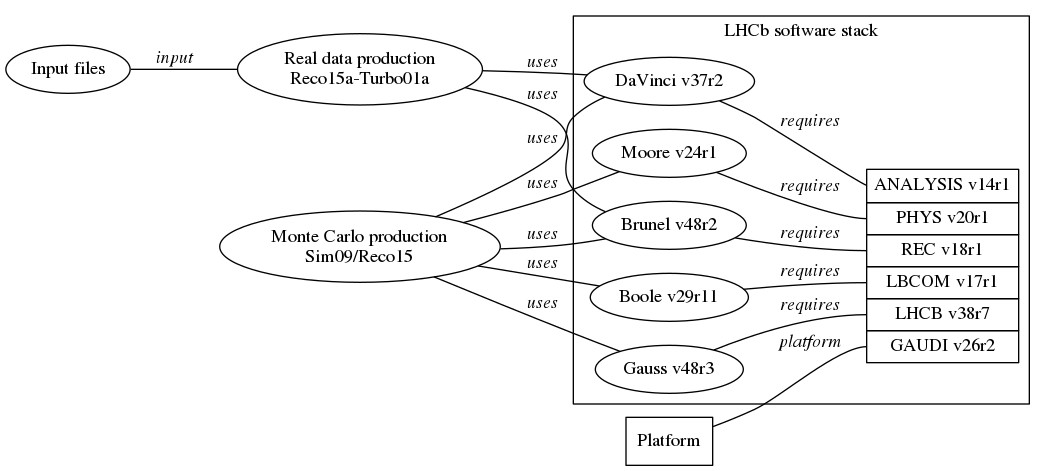
\includegraphics[width=\textwidth]{img/dbstruct}
    \caption{The graph database schema. }
    \label{fig:str}
    \end{figure}
    


\subsection{Application Programming Interface API}

The API to the LHCb graph database is implemented in \emph{py2neo} which is a client library and toolkit for working with \emph{Neo4j} from within Python applications and from the command line. We use the Representational State Transfer (REST)~\cite{jakl2005representational} architectural style to create a request/response mechanism between the server and the client. The data retrieved directly from the database is returned in JSON format. Some of the functions are listed below:

\begin{itemize}
    \item {\bf{ \verb|getProductionSequence(ID)|}} Returns a \emph{Production} entity with the given \emph{ID} number.
    \item {\bf{ \verb|listProjects()|}} Returns the list of \emph{Projects}.
    \item {\bf{ \verb|listPlatforms(Project)|}} Lists the suitable \emph{Platforms} for the given \emph{Project}.
    \item {\bf{ \verb|listRequirements(Project)|}} Lists the required modules for the given \emph{Project}.
\end{itemize}

\subsection{Web portal}

The graph database is connected to a \emph{Django} web server and made available for the users as a web portal. Django is a high-level, open source Python Web framework that encourages clean and pragmatic design of the web applications~\cite{holovaty2009definitive}.

The web portal allows browsing through the LHCb data production and software information. It implements a search engine for this metadata, and it is meant to recommend the latest streaming to the users. In addition, it should promote the LHCb data preservation and provide a comprehensive user guide for analysis documentation and preservation.

\iffalse
\begin{figure}[h]
    \centering
    \includegraphics[width=0.9\textwidth]{img/slide1}
    \caption{Appearance of the web page}
    \label{fig:webp}
\end{figure}
\fi
